\documentclass[amsmath,preprintnumbers,10pt,nofootinbib,prl,twocolumn]{revtex4-1}
\usepackage{amsbsy}
\usepackage{amssymb}
\usepackage{graphicx}
\usepackage{color}
\usepackage{subfigure}
\usepackage{physics}
\usepackage{soul}
\usepackage{color}
\usepackage{bm}
\usepackage[normalem]{ulem}

%\newcommand{\Tr}{\text{Tr}}
\newcommand{\Ai}{\text{Ai}}
\newcommand{\Bi}{\text{Bi}}
\newcommand{\Real}{\text{Re}}
\newcommand{\Imag}{\text{Im}}

\usepackage{verbatim}
\usepackage{natbib}
\bibliographystyle{apsrev4-1}
\begin{document}
\title{Dissipation induced transitions in two dimensional elastic membranes}
\author{Michael Nguyen$^{1,2}$, Suriyanarayanan Vaikuntanathan$^{1,2}$} 
\affiliation{$^1$The James Franck Institute, The University of Chicago, Chicago, IL,}
\affiliation{$^2$ Department of Chemistry, The University of Chicago, Chicago, IL.}
\begin{abstract}
Stochastic thermodynamics provides a useful set of tools to analyze and constrain the behavior of far from equilibrium systems. In this paper, we report an application of ideas from stochastic thermodynamics to the problem of membrane growth. Non-equilibrium forcing of the membrane can cause it to buckle and undergo a morphological transformation. We show how ideas from stochastic thermodynamics, in particular a recent application to self-assembly, can be used to phenomenologically describe and constrain the parameters required to excite morphological changes during a non-equilibrium growth process.

\end{abstract}
\maketitle 

Non-equilibrium forces can potentially provide new routes to modulate self-assembly and organization~\cite{Battle604,Lan2012,Mehta2012,Whitelam2014}. In biophysical contexts, it has been established that non-equilibrium forces play a crucial role in suppressing rogue fluctuations and enhancing fidelity of molecular recognition~\cite{Hopfield1974,Mehta2012,Murugan2012,Murugan2016,Vaikunt2017}, support robust oscillations crucial for the maintenance of circadian rhythms~\cite{Barato2015}, and drive sensory adaptation processes~\cite{Lan2012,Mehta2012}. Non-equilibrium forces also play an important role in modulating cell shape and cell membrane fluctuations~\cite{McMahon2005, Turlier2016}. For instance, local changes in surface tension or lateral pressure due to a spontaneous assembly of membrane proteins have been known to induce instabilities in membrane fluctuations~\cite{Stachowiak2012, Chen2016,Rangamani2014,Leibler1986}. Such instabilities have been implicated as important precursors during cell division~\cite{McMahon2005}. Non-equilibrium fluctuations are also important in cases where the cell membrane interacts with growing actin filaments. The important role played by such interactions in regulating the organization of the membrane has been well established ~\cite{Gowrishankar2012,Weichsel2016}.
\begin{figure}[tbb]
\centering
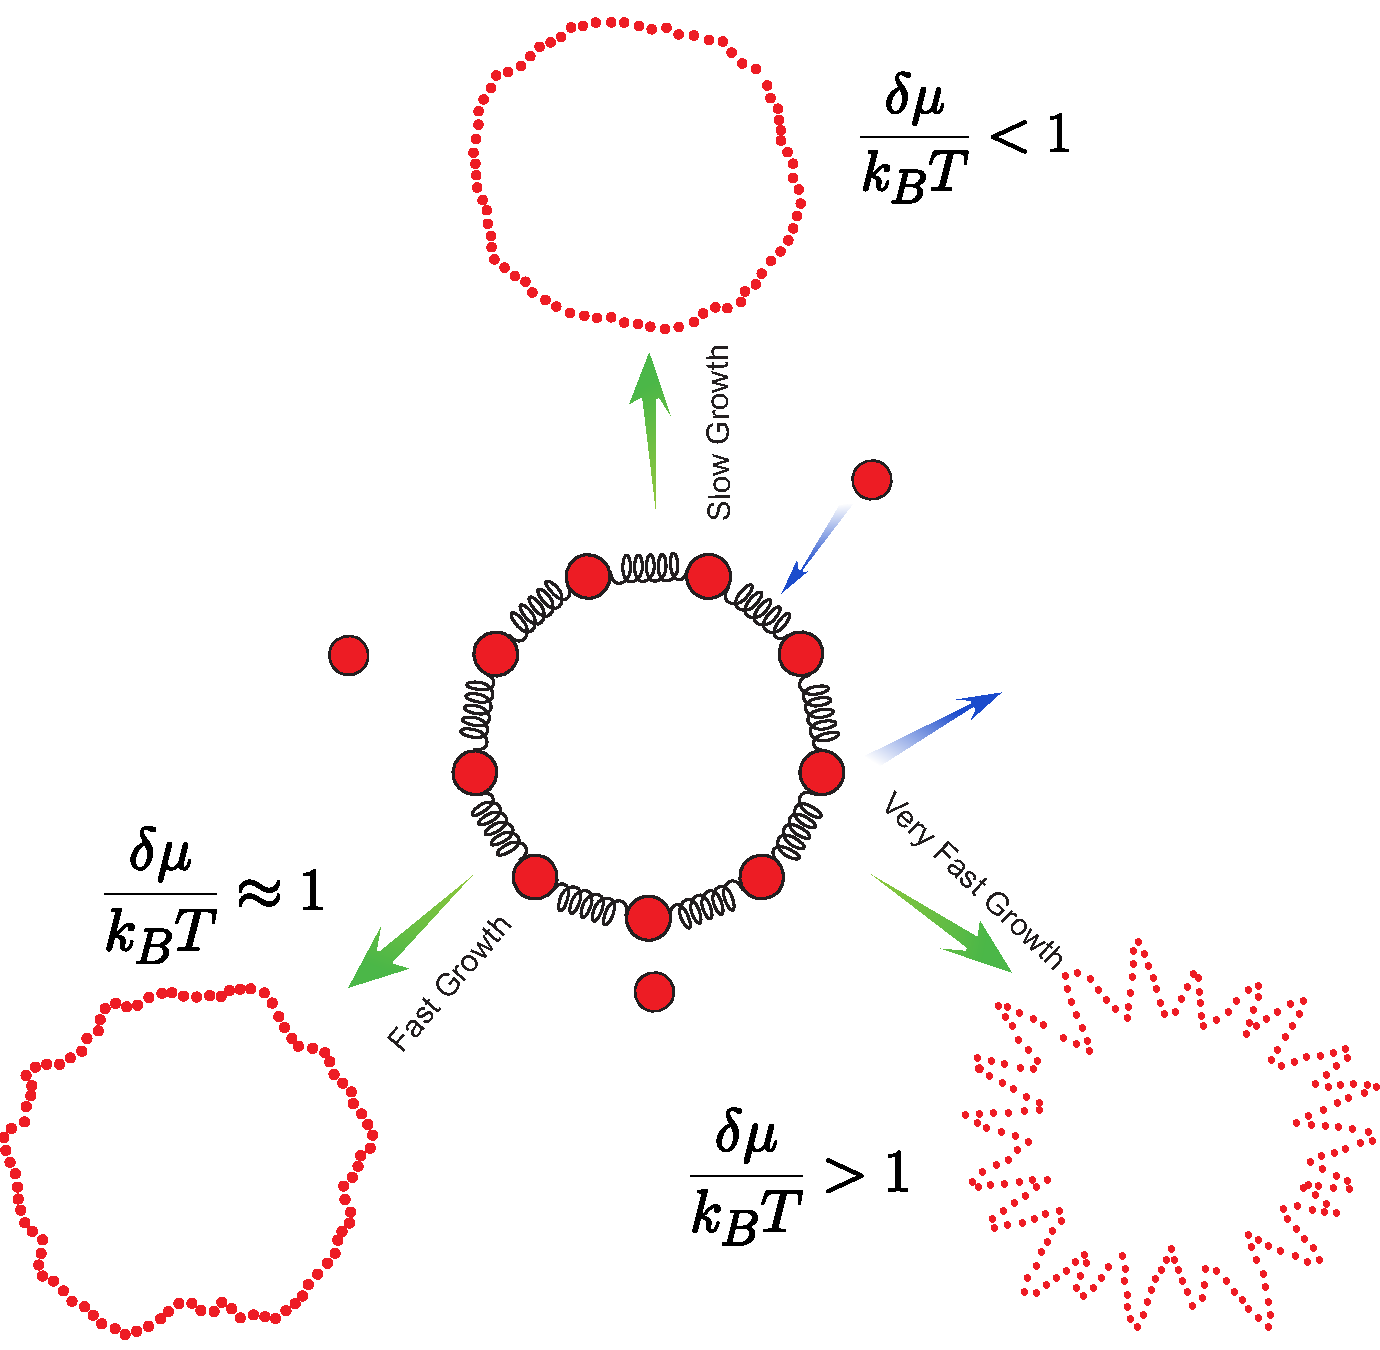
\includegraphics[scale=0.35]{particleinaringschematicFig1.pdf}
\caption{Schematic of the growing assembly. When the assembly grows slowly, its shape remains circular (top figure). As the assembly grows faster, it shape becomes more distorted (lower left) and ultimately it buckles into a star-shaped morphology (lower right).} \label{fig:phases}
\end{figure}


Unlike the behavior and characteristics of equilibrium systems, general principles governing fluctuations about a steady state or the steady state itself in far-from-equilibrium conditions are just being discovered. In particular, the field of stochastic thermodynamics has provided a promising framework to study non-equilibrium systems in mesoscopic scale~\cite{Seifert2012}. The ideas of stochastic thermodynamics have been productively used to elucidate tradeoffs between energy consumption and organization in biochemical reaction networks~\cite{Barato2015,Murugan2016,Vaikunt2017}, self-propelled or driven colloids~\cite{Ganguly2013, delJunco2018,Dasbiswas2017}, and molecular motors~\cite{Gaveau2010, Seifert2011}. Previously, we have also shown how stochastic thermodynamics can be used to derive general design principles for self-assembly~\cite{Nguyen2016}. 


In this letter, we use the framework of stochastic thermodynamics to investigate non-equilibrium growth and morphological changes in a model elastic membrane~\cite{Drasdo2000, Ramaswamy2000,Rao2001,Solon2006,Hannezo2011,Fisher1989,Fisher1989a,Rudnick1991,Rajesh2008,Nelson2009}. Our central results show how an application of stochastic thermodynamics to such systems can provide bounds on the parameters required to renormalize material properties and excite morphological transformations in the membrane system. Our bounds are thermodynamic in nature and depend minimally on the kinetic details of the process chosen. While a detailed kinetic model can indeed be written down to explain the phenomenology observed in our non-equilibrium growth simulations, the utility of a thermodynamic bound is that it can identify combinations of parameters that remain important for reorganization irrespective of kinetic details. As such, we anticipate that our work will be useful for uncovering minimum sets of energetic requirements for driving more complex classes of reorganization events in model membrane systems~\cite{Zwicker2017}. 

Our model consists of two-dimensional particles connected by elastic springs in a ring geometry (Fig~\ref{fig:phases})~\cite{Fisher1989,Fisher1989a,Rudnick1991,Rajesh2008,Nelson2009}. The interactions between particles are chosen such that the fluctuations of the ring at equilibrium can be described by specifying a surface or a line tension and a bending rigidity. The ring assembly is allowed to exchange particles with a reservoir. The chemical potential of the reservoir controls the growth rate of the ring assembly and sets the non-equilibrium driving force in this system.

\textbf{The model was first used by Leibler, Singh, and Fisher~\cite{Fisher1989} who used this model to gain more insights into membrane behaviors.  Their paper then inspired many following papers~\cite{Fisher1989a,Rudnick1991,Rajesh2008,Nelson2009} which use similar models to study membranes with both analytical results and simulations.} Despite its apparent simplicity, this elastic model possesses many features~\cite{W.Helfrich1973,Fisher1989,Fisher1989a,Rudnick1991,Ramaswamy2000,Rao2001,Solon2006,Rajesh2008,Hannezo2011,Loubet2012,Nelson2009} characteristic of three-dimensional membranes and can be used to obtain insights into how morphological changes in such systems can be excited under a non-equilibrium driving force. Indeed, as we describe below, our numerical analysis shows that the effective surface tension and bending rigidity of the elastic ring get modified under non-equilibrium growth conditions. Further, beyond a critical chemical potential driving force, the effective surface tension of the elastic ring is renormalized to zero and the elastic ring exhibits a buckling instability and undergoes a non-equilibrium morphological transformation (Fig~\ref{fig:phases}). Such instabilities have been observed in experiments investigating the growth of model lipid membranes \cite{Solon2006} and can potentially have implications for biophysical processes such as membrane fission and endocytosis. \textbf{In addition, our preliminary results of the 3D membrane model confirm that many of these characteristics such as renormalization of surface tension and bending rigidity, and instability at high drive do carry over (see SI for details). Regardless of the model simplicity, it is not a trivial task in writing down hydrodynamics equations description to describe its behavior. Thus, in this letter, we would like to propose another approach using the principles of thermodynamics to write down thermodynamics bounds with relative ease that can be used to predict the renormalization of the surface tension of the membrane by non-equilibrium drive.}


Using ideas from stochastic thermodynamics, we provide a thermodynamic prescription for how the surface tension and bending rigidity are modified by the non-equilibrium forces (Eqs.~\ref{eq:firstbound} and~\ref{eq:secondbound}). The thermodynamic prescription only requires information about the magnitude of the non-equilibrium chemical potential driving force, the equilibrium surface tension and bending rigidity, the average rate of growth, and fluctuations in the average rate of growth. This thermodynamic prescription was first developed by us in~\cite{Nguyen2016} in the context of different self-assembly problems and is otherwise insensitive to any of the kinetic details used in the growth process. This thermodynamic theory provides bounds on the energetic requirements to induce morphological transformations such as the above described non-equilibrium buckling transition (Fig.~\ref{fig:PhaseDiagram}). \textbf{To gain better insights to the prescription, we think it is more beneficial to give a phenomenological argument on its validity. We have also provided a detailed proof for the prescription on the SI for interested readers.}
We now describe the specifics of the elastic model, phenomenology observed in the non-equilibrium growth process, and how an application of ideas from stochastic thermodynamics can explain this phenomenology. 

%We hope these results will elucidate the energy requirements for achieving processes reminiscent of cell division in biology and will also clarify how non-equilibrium forces can be used as an effective knob for tuning fluctuations in many body condensed systems.

\begin{figure}[tbb]
\centering
\includegraphics[scale=0.29]{scalingindependentofsizeFig2.pdf}
\caption{Power spectrum of interfacial fluctuations at equilibrium. For small wavevectors, q, $|\delta h(q)|^2\propto q^{-2}$ while $|\delta h(q)|^2\propto q^{-4}$ at high q in agreement with expectations Eq.~\ref{eq:HelfrichFT}. The data here is for $k_s=4$ and $k_\theta = 6$. The diamond symbols are fluctuations of the assembly with 200 particles. The square symbols are fluctuations of the assembly with 500 particles. The circle symbols are fluctuation of the assembly with 1000 particles. Because the fluctuations here follow the Helfrich Hamiltonian, its standard deviation is exactly equal to its average magnitude due to the exponential nature of the distribution.} \label{fig:HelfrichScaling}
\end{figure}

\begin{figure}[tbb]
\centering
\includegraphics[scale=0.34]{newscalingacrossFig3.pdf}
\caption{Power spectrum of interfacial fluctuations at different $\delta\mu$. Fitting these curves to Eq.~\ref{eq:HelfrichFT} allows to obtain estimates of $\gamma_{\rm eff}$ and $\kappa_{\rm eff}$ as described in the text. This analysis reveals that $\gamma_{\rm eff}$ decreases with increasing $\delta\mu$. The data here is for $k_s=4$ and $k_\theta = 6$.} \label{fig:Helfrich}
\end{figure}




Our specific model consists of particles in a ring like geometry interacting according to the Hamiltonian, 
\begin{equation}
\label{eq:Halmitonianl}
E=\sum_i^N{\frac{k_s}{2}(l_{i,i+1}-l_0)^2+k_\theta(\theta_i-\pi)^2}\,,
\end{equation}
where $l_{i,i+1}$ is the distance between particle $i$ and particle $i+1$, $l_0$ is the equilibrium distance and $\theta_i$ is the angle that particle $i$ makes with its neighbors. The growth dynamics of the Monte Carlo simulation is detailed in SI Fig S1. In short, in each Monte Carlo step, we attempt to add a particle from the bath or remove a random particle from the assembly with equal probability. The protocol used to add particles is specified in SI Fig 1.  Events adding particles to the assembly are accepted with the probability $\rm{min}\{1,e^{(-\Delta E +\mu)/k_B T}\}$ and events removing particles from the assembly are accepted with the probability $\rm{min}\{1,e^{(-\Delta E -\mu)/k_B T}\}$. Here, the parameter $\mu$ can be regarded as the chemical potential of monomer units in the bath and $k_B T$ sets an energy scale. From now on, we will set $k_B T = 1$ for simplicity. 

The rate of growth of the elastic assembly can be tuned by varying the parameter $\mu$. Specifically, we find that there exists a \textit{coexistence} value of $\mu$, $\mu_{coex}$ at which the assembly does not grow on average. The system is at equilibrium with its surroundings for this value of $\mu$. In the rest of the manuscript, we use the term equilibrium to refer to conditions where $\mu =\mu_{coex}=\mu_{eq}$, and the term non-equilibrium to refer to conditions where $\mu > \mu_{eq}$. 

For values of $\mu$ above the coexistence value $\mu_{eq}$, the system is driven away from equilibrium and the elastic ring polymer starts to grow. When $\delta\mu/k_BT \equiv (\mu-\mu_{eq})/k_B T$ is small, the elastic assembly grows slowly and roughly retains its circular shape. With increasing $\delta\mu/k_B T$, the elastic assembly grows faster; its shape becomes more distorted and ultimately buckles resulting in spikes growing out of the circle as shown in Fig.~\ref{fig:phases}. 

To study the above mentioned morphological changes(Fig.~\ref{fig:phases}), we examine how the fluctuations of the elastic ring polymer are modified as a function of its growth rate. Specifically, to simplify the discrete Fourier transform, we use an approximation that the distance between the particles are uniform which equal $\langle l \rangle=\frac{L}{N}$. Here L is the circumference of the assembly and N is the number of particle. We then measure fluctuations in $\hat{h}(x_n)$ where $x_n\equiv n\langle l \rangle$, $n$ labels the particles in the elastic ring and $\hat{h}(x_n)$ denotes the deviation of the distance of a particle from the center of the assembly from the average radius of the elastic assembly, $\hat{h}(x_n)\equiv h(x_n) -\langle h \rangle$. The ensemble over which the fluctuations are measured was constructed by initiating simulations with a certain initial elastic assembly nucleus with size $N_0$ and allowing the nucleus to grow for a time $t_{\rm measure}$. In order to ensure that our results are not affected by choices of $N_0$ and $t_{\rm measure}$, simulations with multiple values of $N_0$ and $t_{\rm measure}$ were considered. In ensembles constructed in this manner, we measured $\langle |\delta h(q)|^2 \rangle$ where $\delta h(q)$ is the Fourier transform of the radial fluctuations defined with the convention: $\hat{h}(x_n)=\frac{1}{\sqrt{N}}\sum _q \delta h(q) \exp(iqx_n), q = \frac{2\pi m}{N\langle l \rangle}, m = 1, 2,...,N$. Here N is the number of particles in the elastic assembly. 

At or close to equilibrium, $\delta \mu /k_B T \ll 1$, by measuring fluctuations and averaging over the above described ensembles, we find that $\langle |\delta h(q)|^2 \rangle$ scales likes $q^{-2}$ in the low $q$ regime and scales like $q^{-4}$ in the high $q$ regime (Fig.~\ref{fig:HelfrichScaling}). This suggests that 
at equilibrium, the fluctuations of the elastic ring can be effectively described using the Helfrich Hamiltonian~\cite{W.Helfrich1973}:
\begin{equation}
E_{eq}=\int \left \{\frac{\gamma}{2} (\nabla \hat{h})^2+  \frac{\kappa}{2} (\Delta \hat{h})^2\right \} dx.
\label{eq:Helfrich}
\end{equation}
Motivated by the scaling in Fig.~\ref{fig:HelfrichScaling}, we refer to the parameter $\gamma$ as an effective surface tension and the parameter $\kappa$ as an effective bending rigidity. At equilibrium, $k_s$ is inversely proportional to $\gamma$ and does not affect $\kappa$. On the other hand, increasing $k_\theta$ seems to increase $\gamma$ and decrease $\kappa$. We stress again that we are defining these elastic constants, $\gamma$ and $\kappa$ in the context of the ensembles defined above. 

Even as the assembly starts to grow, Fig.~\ref{fig:Helfrich} shows that the radial fluctuations are still described by an effective Helfrich Hamiltonian with renormalized surface tension and bending rigidities $\gamma_{\rm eff}$ and $\kappa_{\rm eff}$. Indeed, Fig.~\ref{fig:Helfrich} shows that the average $\langle |\delta h(q)|^2 \rangle$ is well described by 
\begin{equation}
\langle |\delta h(q)|^2 \rangle \propto \frac{k_B T}{(\gamma_{\rm eff} q^2 + \kappa_{\rm eff} q^4)}\,,
\label{eq:HelfrichFT}
\end{equation}
in accordance with Eq.~\ref{eq:Helfrich} with renormalized effective surface tension and bending rigidity values. Closer inspection of the effective surface tension and bending rigidity extracted from Fig.~\ref{fig:Helfrich} shows that the effective surface tension,$\gamma_{\rm eff}$ decreases as $\delta \mu$ is increased, dropping to $\gamma_{\rm eff}\approx 0$ at a critical value of $\delta \mu=\delta \mu_c$ (Fig.~\ref{fig:HelfrichInstability}). Beyond this point, the elastic assembly buckles and undergoes a morphological transformation to ring populated by \textit{}{spikes}. The number of spikes appearing in a process is proportional to the initial size of the assembly and $\delta\mu$ (see Fig. 4) and remains constant during the growing period. 
Reflecting the diminished effective surface tension cost under non-equilibrium conditions, the configurations with spikes allow the system to grow with minimal penalties for stretching. The bending rigidity does not seem to change by a large amount as indicated in Fig.~\ref{fig:Helfrich}. We again note that we have extracted the effective renormalized values of the surface tension and bending rigidity for multiple values of initial size $N_0$ and simulation time $t_{\rm measure}$. We find that to a good numerical approximation, the effective elastic constants, $\gamma_{\rm eff}$, $\kappa_{\rm eff}$ and values of the parameters $\mu_{coex}$, and $\delta \mu_c$, are time and size independent in all our simulations as shown in Fig.~\ref{fig:HelfrichScaling}. 

%We again note that we performed numerical simulations with multiple initial sizes $N_0$ and multiple choices of $t_{\rm measure}$. The values of $\delta \mu$, $\gamma_{\rm eff}$. $\kappa_{\rm eff}$, $\delta \mu_c$ were independent of $N_0$ and $t_{\rm measure}$ in our numerical simulations. 

\begin{figure}[tbb]
\centering
\includegraphics[scale=0.25]{lobefork4ktheta6new2Fig4.pdf}
\caption{Phase diagram for data at $k_s=4$ and $k_\theta = 6$. As $\delta\mu$ is increased, the effective surface tension $\gamma_{\rm eff}$ decreases eventually reaching $\gamma_{\rm eff}\approx 0$ for $\delta\mu \approx 1.0$.  Increasing $\delta \mu$ beyond this value induces a morphological change to a configuration with spikes. The data was obtained with $N_0=200$. The red curve in the figure represents the surface tension $\gamma$ of the assembly before the instability. The error bar represents the 95\% confidence interval from fitting.After the instability, $\gamma$ is negative and cannot be measure using the Fourier transform technique. We then use the number of spikes (the blue curve) in the assembly, which can be used to infer the instabilities' wavelength, to indicate the systems at different drive post the instability. The blue curve in the figure represents the number of spikes} \label{fig:HelfrichInstability}
\end{figure}

We now use ideas from stochastic thermodynamics to understand the trade-offs between non-equilibrium driving (as characterized by $\delta \mu$) and morphological changes in the structure of this elastic ring system (as characterized by the renormalized constants $\gamma_{\rm eff}$ and $\kappa_{\rm eff}$). We begin by noting that our numerical results suggest that the even when the elastic ring is not at equilibrium, its fluctuations can be described in terms of an effective energy landscape, (Fig.~\ref{fig:Helfrich}). In this case, the entropy of the growing elastic system at a time $t$ can effectively be written down as~\cite{Nguyen2016,Esposito2012}
\begin{equation}
\label{eq:entropysystem}
 TS=\left\langle N \right\rangle_t \frac{-F_{\mathit{eff}} + \langle E_{\mathit{eff}} \rangle _N}{N}\,,
\end{equation}
where $E_{\mathit{eff}}$ is the effective elastic energy of a configuration in terms of the renormalized material parameters $\gamma_{\rm eff}$ and $\kappa_{\rm eff}$, $F_{\mathit{eff}}$ is the Helmholtz free energy appropriate to $E_{\mathit{eff}}$, $\langle...\rangle_N$ is the average of all microscopic configurations of the assembly at size $N\gg 1$ and $\langle N \rangle_t$ is the average size of the elastic ring after it has been allowed to grow for a time $t$. Since $d\langle N \rangle_t/dt > 0$ under non-equilibrium conditions $\delta\mu >0$, the entropy of the system changes as a function of time. 

We can similarly compute the change in the entropy of the bath as it supplies monomers to the elastic assembly and maintains constant chemical potential conditions. Specifically, in the limit that the bath size is much larger than the size of any elastic assembly, the change in entropy of the bath after a time t, $\Delta S_{bath}$, can be written as :
\begin{equation}
\label{eq:entropybath}
 T\Delta S_{bath}=-\left\langle N \right\rangle_t \frac{-F_{\mathit{eq}} + \langle E_{\mathit{eq}} \rangle _N-N\delta\mu}{N}
\end{equation}
By combining Eq.~\ref{eq:entropysystem} and Eq.~\ref{eq:entropybath}, we can write down the total entropy of the process, which must be nonnegative according to the second law of thermodynamics~\cite{Esposito2012}:
\begin{equation}
\begin{split}
\label{eq:entropytotal}
\frac{dS_{total}}{dt}&=\frac{dS}{dt} +\frac{dS_\mathit{bath}}{dt}\\
&= \frac{d\langle N\rangle}{dt}\left ( \delta\mu-\langle\epsilon_{diss}\rangle \right) \geq 0
\end{split}
\end{equation}
Here $\langle\epsilon_{diss}\rangle=\left (\left\langle E_{eq}-E_{\mathit{eff}}\right\rangle _N-\left ( F_{eq}-F_{\mathit{eff}}\right )\right )/N$. $\langle\epsilon_{diss}\rangle$ can be thought as the minimum work required to transform the energy landscape of the system from $E_{\rm eq}$ to $E_{\rm eff}$ using a driving force. The driving force here can come from many sources such as activity of matters, mechanical works. In this letter, the driving force here is the extra chemical potential we put into the bath.  For a growing system, $\frac{d\langle N \rangle}{dt}$ is positive thus reducing the second law to:
\begin{equation}
\label{eq:firstbound}
\delta\mu-\langle\epsilon_{diss}\rangle\geq0
\end{equation}

In addition, using the recently derived uncertainty relations that relate the entropy production to the current fluctuations of the system \cite{Barato2015, Gingrich2016,Nguyen2016}, we can propose a tighter bound:
\begin{equation}
\label{eq:secondbound}
\delta\mu-\langle\epsilon_{diss}\rangle\geq\frac{v k_B T}{D}\, 
\end{equation}
where $v=\frac{d\langle N\rangle}{dt}$ is the growth rate of the assembly, and $D=\lim_{\tau\to\infty}\frac{\langle\Delta N^2\rangle}{2\tau}$  is the diffusion constant of the size fluctuations of the assembly.

The bounds in Eq.~\ref{eq:firstbound} and Eq.~\ref{eq:secondbound} constrain the allowed values of $\gamma_{\rm eff}$ and $\kappa_{\rm eff}$ given $\delta \mu$, the equilibrium elastic constants $\gamma_{\rm eq}, \kappa_{\rm eq}$ and the ratio $vk_BT/D$. In deriving Eq.~\ref{eq:firstbound} and Eq.~\ref{eq:secondbound}, the main approximation we made was to ignore correlations between fluctuations in the number density and fluctuations in the configurations. In Ref.~\cite{Nguyen2016}, using a one dimensional polymer growth model, we showed that this approximation is fairly reasonable. 
In the limit of slow growth where the effective elastic constants are minimally renormalized, $\delta\mu \gg \epsilon_{diss}$, Eq.~\ref{eq:secondbound} reduces to the following statement of linear response,
\begin{equation}
\label{eq:linearresponse}
\delta\mu=\frac{v k_B T}{D}
\end{equation}
In Fig.~\ref{fig:LinearResponse} we numerically verify that our simulations at two different sizes indeed satisfy this linear response condition, Eq.~\ref{eq:linearresponse} when $\delta \mu/k_B T \ll 1$. Further, Fig.~\ref{fig:LinearResponse} also shows that $\delta \mu \geq vk_BT/D$ in agreement with Eq.~\ref{eq:secondbound} in the slow driving limit.  


\begin{figure}[tbb]
\centering
\includegraphics[scale=0.3]{linearresponseregimeFig5.pdf}
\caption{$\frac{v}{D}$ vs. $\delta\mu$. In this case, $k_BT$ is set to 1. The dark line is predicted from linear response. The error bar represents the 95\% confidence interval from the fit Eq.~\ref{eq:linearresponse}.} \label{fig:LinearResponse}. The blue dot is from the assemblies of 200 particles, while the orange dot is from the assemblies of 500 particles. The two measurements overlaps with some minor error. \end{figure} 

We will now use Eq.~\ref{eq:secondbound} to understand how $\gamma_{\rm eff}$ can be controlled by tuning $\delta \mu$. As first approximation, given the relatively slow renormalization of the bending rigidity Fig~\ref{fig:Helfrich}, we will set $\kappa_{\rm eff}=\kappa_{\rm eq}$. Within this approximation (see SI for details), we will obtain: 
\begin{equation}
\label{eq:epsilonexpress}
 \langle\epsilon_{diss}\rangle =\frac{k_{B}T\lambda}{4\pi}\left ( \frac{(\gamma_{\rm eff} + \gamma_{\rm eq})\phi-2\sqrt{\gamma_{\rm eff}\gamma_{\rm eq}}\phi^*}{\sqrt{\gamma_{\rm eff} \kappa_{\rm eq}}}-\frac{2\pi \xi}{\lambda} \right)
\end{equation}
Here $\phi=\arctan(\frac{2\pi\sqrt{\kappa_{\rm eq}}}{\lambda\sqrt{\gamma_{\rm eff}}}), \phi^*=\arctan(\frac{2\pi\sqrt{\kappa_{\rm eq}}}{\lambda\sqrt{\gamma_{\rm{eq}}}})$, $\xi=\ln(\frac{\gamma_{\rm{eq}}\lambda^2+4\pi^2\kappa_{\rm eq}}{\gamma_{\rm eff}\lambda^2+4\pi^2\kappa_{\rm eq}})$, and $\lambda$ is the smallest wavelength allowed by the assembly which we will take to be $l_0$. Using this expression for $\epsilon_{diss}$, Eq.~\ref{eq:firstbound} and Eq.~\ref{eq:secondbound} can be used to predict bounds on how $\gamma_{\rm eff}$ changes with the non-equilibrium driving $\delta \mu$. These predictions are plotted in Fig.~\ref{fig:PhaseDiagram} alongside the scaling of $\gamma_{\rm eff}$ with $\delta \mu$ extracted from simulations. 

\begin{figure}[tbb]
\centering
\includegraphics[scale=0.28]{boundscheckFig6.pdf}
\caption{Thermodynamic bounds on the surface tension as a function of the non-equilibrium driving force $\delta\mu$. The bound stipulated by the blue curve is from Eq.~\ref{eq:firstbound}. The bound stipulated by the orange curve is from Eq.~\ref{eq:secondbound}. The green curve is obtained by measuring $\gamma_{\rm{eff}}$ from simulations and is consistent with the bounds specified by Eq.~\ref{eq:firstbound} and Eq.~\ref{eq:secondbound}. These bounds provide rough estimates for the energetic costs required to modify the morphology and fluctuations in the elastic membrane. }\label{fig:PhaseDiagram}
\end{figure}

As expected from linear response theory, the bound in Eq.~\ref{eq:secondbound} agrees very well with simulation results close to equilibrium. \textbf{ Away from equilibrium, Eq.~\ref{eq:secondbound} indeed provides a lower bound for $\delta \mu$. As we go very far from equilibrium and approach the instability $\gamma_{\rm eff}\approx 0$, where linear response should fail (see Fig.~\ref{fig:LinearResponse}), our bounds still hold and can give a quantitative predictions on the point of instability. Fig.~\ref{fig:PhaseDiagram} shows how ideas from stochastic thermodynamics can be used to predict how material properties such as the surface tension, can be modified in the presence of non-equilibrium forces.} It also provides a thermodynamic lower bound for the minimum non-equilibrium driving force $\delta \mu$ required to obtain $\gamma_{\rm eff}\sim 0$ and induce morphological transformations in the system. 


The role played by non-equilibrium forces in biological processes such as those responsible for modulating cell shapes and dynamics is well established~\cite{McMahon2005,Stachowiak2012,Chen2016,Turlier2016,Rao2001,Solon2006}. Using the formalism of stochastic thermodynamics, we have probed the tradeoffs between energy consumption and organization in a model non-equilibrium membrane growth process. \textbf{Although in this letter we have limited our driving force to an extra chemical potential, our prescription we provided can be extended to other non-equilibrium drive such as proteins-inducing membranes.} Given the minimal kinetic detail required by our effectively thermodynamic bounds, we anticipate that our results will find broad applicability in more complex varieties of membrane reorganization processes in synthetic~\cite{Zwicker2017} and biological systems. 

%The validity of the above argument lies on the assumption that an entropy production term can be constructed for such process. In addition, we have also assume that the system can be described using an effective Helfrich Hamiltonian and this simply might not be the case. For the second part, we want to stress that at this time, we have only used very little information on the system: only the means amplitude of the mode which is zero and their variance. Without more information on the system, it would not be optimal to attempt the above approach with more complicated distribution. As for the first part, in general, in order to derive an expression for the entropy production of the process, one has to construct an Markov model with master equation or an Stochastic Differential Equation which by no mean a trivial task. Here, by using the approach that we previously developed, we are able to write out an expression for the entropy production with minimal information. However, to further illustrate that it is possible to describe our system with an entropy production, we have constructed a Markov model that can describe our system qualitatively and derived an entropy production term from it. 
%\begin{figure}[tbb]
%\centering
%\includegraphics[scale=0.33]{markovmodelparticleinaringver2.pdf}
%\caption{Schematic of our Markov network. The vertical rungs represents the amplitude of our modes while the horizontal line represents the number of particle. The number of nodes here are just for illustration and does not reflect the actual number of nodes that increase with system size} \label{fig:markov}
%\end{figure}

%In our model, working in Fourier space, we imagine a Markov network with nodes describing the fluctuation of $\delta h(q)$ of the system (Fig 8). The vertical rungs will indicate the amplitude of the modes while the horizontal line describe the system size. Because the number of modes is proportional to the number of particles, the number of nodes our Markov model can access also increases with the assembly size. In fact, the state space accessible by our model scales like $\mathbb{R}^N$. Adding a particle is like introducing a small wavelength mode to the assembly in which the amplitude, $|h|^2$ , is chosen according to $P\propto  \textrm{Exp}[-\Sigma\kappa q^4 |h|^2]$. The acceptance rate of such configuration is $\mathit{Min}[ \textrm{Exp}[(-\Sigma\gamma q^2 |h|^2+N\mu)],1]$. We then look at the steady state mode probability distribution of the assembly and attempt to remove it with accepting rate: $\mathit{Min}[\textrm{Exp}[(\Sigma\gamma q^2 |h|^2-N\mu)],1]$.  Because the modes of the system keep increasing with the assembly size, the transition rate of our Markov model also depends on time. Specifically, for each new mode, we have to add an extra term $-\gamma q^2 |h|^2+\mu$ to the addition acceptation rate and $\gamma q^2 |h|^2-\mu$ to the removal acceptance rate. Since we only care about the steady state of the process, we can approximate our Markov process with a Poisson Process \cite{Maes2008} with an effective arrival rate $\lambda$ which like the acceptance rates of the Markov process has to increase with $N$ as well. The probability at certain time, t, for the arrival of a particle of a Poisson process is: $\lambda t \textrm{Exp}(-\lambda t)$. Thus, if one cannot increase the rate $\lambda$, the time has to increase to compensate for the effect of adding more modes into the system.  In order words, when the assembly only has 1 particle and it would take only certain time $t$ to add a particle. For a system with N particle, one would require $Nt$. This is reflected in the square root growth rate of our simulations.  With a few line of algebra, it can be shown that the steady state distribution of this model is only in Gaussian form when it is at equilibrium and at very far from it.  In addition, this model cannot give an instability. However, it does give the same scaling of $|h^2|$ as our simulations that is as one increase $\delta\mu$, the surface tension $\gamma$ will decrease.
The authors acknowledge support from NSF DMR-
MRSEC  1420709, NSF GFRP and the  University  of  Chicago
 
\bibliography{References02232018}
\end{document}